\documentclass{standalone}

\usepackage{tikz}
\usepackage{graphicx}
\pagestyle{empty}

% INT_AY22_L35-Fig02_Wire_approx.png

\begin{document}
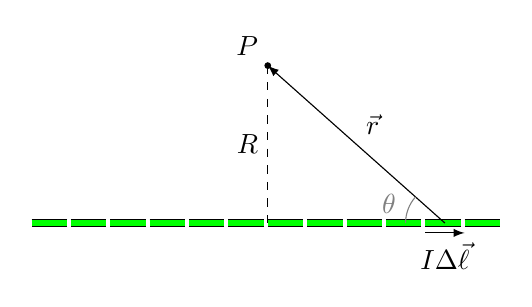
\begin{tikzpicture}[> = latex]

	% Definitions
	
	\def\L{6}		% Wire length
	\def\N{12} 		% Number of wire segments
	\def\R{2}		% Distance to observation point
	
	% Wire segments
	
	\foreach \n in {0, 1, ..., 11}
		\draw [double = green, double distance = 2 pt] ({\n * \L / \N}, 0) -- ({(\n + 0.9) * \L / \N}, 0);
		
	% Observation point P
	
	\filldraw (0.5 * \L, \R) circle (1 pt) node [above left] {$P$};
	\draw [dashed] (0.5 * \L, \R) -- node [left] {$R$} (0.5 * \L, 0);
		
	% Radius vector
	
	\draw [->] ({(\N - 1.5) * \L / \N}, 0) -- node [above right] {${\vec r}$} (0.5 * \L, 2);
	
	% Length vector
	
	\draw [->] ({(\N - 2) * \L / \N}, -0.125) -- node [below] {$I \Delta {\vec \ell}$} ({(\N - 1) * \L / \N}, -0.125);
	
	% Angle indicator
	
	\draw [thin, gray] ({(\N - 2.5) * \L / \N}, 0) node [above left] {$\theta$} arc (180 : 180 - atan(2 * \R * \N / (\L * (\N - 3))) : {\L / \N});

\end{tikzpicture}
\end{document}